\documentclass[tikz,border=2pt]{standalone}
\usepackage{amsmath}
\usepackage{pgfplots}
\pgfplotsset{compat=1.18}
\usetikzlibrary{arrows.meta}
\begin{document}
% Prisoner's dilemma with v(C,C)=3, v(D,C)=5, v(D,D)=1 and k=2 punishment periods:
% deviating at t gains 5-3=2 once and loses 3-1=2 in t+1 and t+2 (worth 2*delta and 2*delta^2),
% after which play returns to 3.
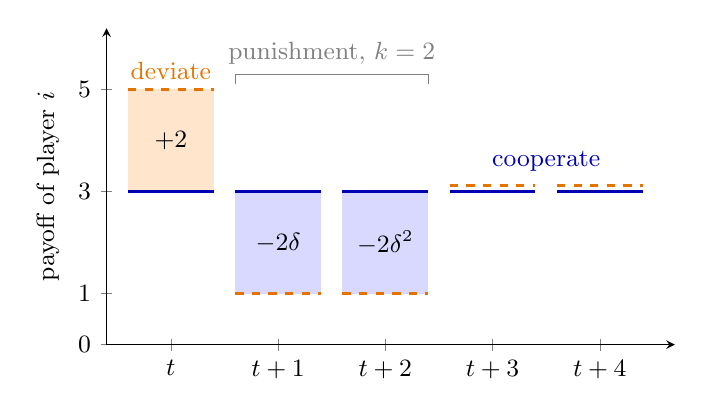
\begin{tikzpicture}[font=\small, >={Latex[length=2mm]}]
  \begin{axis}[width=8.8cm, height=5.6cm, axis lines=left,
      xmin=-0.6, xmax=4.7, ymin=0, ymax=6.2,
      xtick={0,1,2,3,4}, xticklabels={$t$,$t+1$,$t+2$,$t+3$,$t+4$},
      ytick={0,1,3,5}, ylabel={payoff of player $i$},
      clip=false]
    % gain and losses
    \fill[orange!20] (axis cs:-0.4,3) rectangle (axis cs:0.4,5);
    \fill[blue!15] (axis cs:0.6,1) rectangle (axis cs:1.4,3);
    \fill[blue!15] (axis cs:1.6,1) rectangle (axis cs:2.4,3);
    \node at (axis cs:0,4) {$+2$};
    \node at (axis cs:1,2) {$-2\delta$};
    \node at (axis cs:2,2) {$-2\delta^2$};
    % cooperative stream
    \pgfplotsinvokeforeach{0,1,2,3,4}{
      \draw[very thick, blue!70!black] (axis cs:#1-0.4,3) -- (axis cs:#1+0.4,3);}
    % deviation stream
    \draw[very thick, orange!90!black, dashed] (axis cs:-0.4,5) -- (axis cs:0.4,5);
    \draw[very thick, orange!90!black, dashed] (axis cs:0.6,1) -- (axis cs:1.4,1);
    \draw[very thick, orange!90!black, dashed] (axis cs:1.6,1) -- (axis cs:2.4,1);
    \pgfplotsinvokeforeach{3,4}{
      \draw[very thick, orange!90!black, dashed] (axis cs:#1-0.4,3.12) -- (axis cs:#1+0.4,3.12);}
    % labels
    \node[orange!90!black, anchor=south] at (axis cs:0,5) {deviate};
    \node[blue!70!black, anchor=south] at (axis cs:3.5,3.2) {cooperate};
    \draw[gray, thin] (axis cs:0.6,5.1) -- (axis cs:0.6,5.3) -- (axis cs:2.4,5.3) -- (axis cs:2.4,5.1);
    \node[gray, anchor=south] at (axis cs:1.5,5.3) {punishment, $k=2$};
  \end{axis}
\end{tikzpicture}
\end{document}
